\documentclass{article}
\usepackage{amsmath}
\usepackage{hyperref}
\usepackage{graphicx}
\hypersetup{
    colorlinks=true,
    linkcolor=blue,
    filecolor=magenta,
    urlcolor=blue,
}
\usepackage[parfill]{parskip}
\usepackage{bm}

\newcommand{\pw}{p_{\text{win}}}
\newcommand{\pd}{p_{\text{draw}}}
\newcommand{\pl}{p_{\text{lose}}}
\newcommand{\Rw}{R_{W_{\text{adj}}}}
\newcommand{\Rb}{R_{B_{\text{adj}}}}

\begin{document}

\title{Do professional chess players draw too often?}
\author{Tudor Muntianu}
\maketitle

\section*{Disclaimer}
I spent most of my time trying to get the models working. It was a complete nightmare. I thought it was close to working for many hours. Last 1\% took 99\% of the time.
Getting the factor analysis model to work (replacing Smerdon's PCA) took me about 10 hours alone.
Maybe I should have settled for PCA for this draft.
Perhaps I should not have tried to relearn Pyro, a probabilistic programming language written in Python.
That being said, if I had to build this model in R I likely would have ended up using RStan, which is a binding to another PPL, so the model wouldn't have really been in R either.
The data cleaning and manipulation would also have taken me 10x longer since I don't really know R.
Hindsight is 20/20. I think it's on its way, though.

The code (and this writeup) is in a rough state as a result -- by the final draft it will be pretty and commented and clear (despite being in Python).
Similarly, since the model was giving me issues I didn't have compute time to train the model on the whole dataset (which is 4.6M games after cleaning).
Again this will not be the case by the final draft. Everything works though; I have a complete pipeline
that just needs some clean up, some hyperparameters to be adjusted/played with, and to be run to completion.

Also, there are a couple of things I would like to add (or at least investigate) by the final draft:
\begin{itemize}
    \item Dataset of online games (ostensibly less incentive to draw here, more ``naturalistic'' or aggressive gameplay)
    \item Using the factor model to compute an index, comparing to Smerdon's results
\end{itemize}

All code can be found \href{https://github.com/tmuntianu/chessdraws}{here}.

\section{Introduction}

The prevalence of draws in professional chess has been steadily increasing over the past couple decades.
As play becomes more precise and accurate due to extensive computer preparation and analysis,
and as more money enters the sport, winning edges are diminished and players are increasingly
incentivized not to lose.
For instance, at the 2018 World Chess Championship, where Magnus Carlsen played Fabiano Caruana (World No. 1 and No.2 respectively),
all 12 classical time-control games were drawn.
The championship was decided by a rapid chess tiebreaker.
Near-perfect play is not the only factor, however.
Since tournament fates, prize pools, and sponsorship deals hinge on performance, losing is highly undesirable.
So, the popular argument goes, players play for and agree upon too many draws. This opinion is shared by
many strong players and professionals, notably Susan Polgar, a very strong grandmaster who argues that agreed draws should be eliminated from the game.
While some agreed draws are legitimate reflections of drawn game state, others occur when players simply play out opening moves and subsequently agree to draw
to minimize variance. This sort of behavior is most egregious, but it demonstrates the most extreme form of this behavior, making it likely
that playing passively or ``soft-playing'' for draws also occurs.

The question we want to answer is: are draws in high-level chess a result of optimal play?
or are players sacrificing chances to win to reduce variance as a result of external pressures?
Playing ``solid'' chess (i.e., slow, methodical, less aggressive) that lends itself to more draws is not what we are investigating,
but rather if players are playing worse as a result of draw incentives. In other words, are players
playing below their true strengths as a result of playing for draw?
Put even another way, are players are playing to maximize the single-game outcome (i.e., win if possible, draw if losing),
or are players sacrificing performance to reduce their variance?
% From here out, irrational play will be used to refer to this playstyle. This is not technically true, since the payoffs for players are not just winning or losing, but reputation, sponsorships, tournament placement, etc.
% But for the purposes of this paper, playing rationally means playing to maximize the outcome of an individual game, not playing to maximize the real-world consequences.

In this paper the frequency of draws is estimated and compared to existing estimates, namely the very robust Elo rating system used in professional play. We begin by adapting David Smerdon's Fighting Chess Index to generate latent variables representing player behavior and aggression,
then use those latent variables in a simple Bayesian model to estimate the probability of winning, drawing, and losing.
Then, using the Elo rating system, we compute the expected value of the game's outcome, and compare our estimated probabilities to those generated by ratings to determine whether drawing behavior results in poorer results.

\section{Optimal chess}

Given two players $W$ and $B$, we want to know
$p=(p_{\text{win}}, p_{\text{draw}}, p_{\text{lose}})$, where $p_{\text{outcome}}$ is
the probability of $W$ (white) winning, drawing, and losing respectively.

The Elo system, while it does not give a perfect estimate of $p$, does shed some light.

\subsection{Elo ratings}
The Elo rating system gives an excellent estimate of the strength of a player.
With sufficient games played against many opponents, its application to chess produces robust results. All major chess governing bodies (USCF and FIDE) use Elo as their rating system,
chess engines are benchmarked using Elo, and it is used ubiquitously in tournaments to determine seeding and matches.

Given the ratings $R_A$ and $R_B$ of two players $A$ and $B$ respectively, the Elo rating system predicts game outcomes as follows.
\begin{gather*}
    Q_A = 10^{R_A/400}, Q_B = 10^{R_B/400} \\
    E_A = \frac{Q_A}{Q_A+Q_B} \\
    \text{where } E_A = p_{\text{win}} + \frac{1}{2} p_{\text{draw}}
\end{gather*}
It follows from this that $E_A+E_B=1$.

\subsection{Equilibria under Elo assumptions}

The Elo rating system makes an implicit assumption that draw frequency does not directly affect
the expected score $E$, as it does not define $p_{\text{win}}$ directly.

There are infinite solutions to $E = p_{\text{win}} + \frac{1}{2} p_{\text{draw}}$.
Under Elo assumptions players can play solid passive chess and solid aggressive chess,
changing the probabilities of winning and drawing but importantly \textit{not changing}
the total expected value $E$.

This makes any set of strategies chosen by both players a Nash equilibrium under Elo assumptions, since the expected score for any two strategies is equal.
Intuitively, under Elo's system, players can play well
aggressively and they can play well passively; the choice of playstyle will not affect the outcome.

But if players play an overly passive style to achieve more draws,
they decrease their total expected value $E$ to increase $p_{\text{draw}}$.
This is the sort of behavior we are interested in, whether players play
too passively or draw too often \textit{at the expense} of playing optimal chess.

This is Polgar's prediction, as described \href{https://chessdailynews.com/the-700-lbs-gorilla-issue-to-draw-or-not-to-draw/}{here}; i.e., real-world circumstances encourage drawing over playing optimally.
As a result of chess being played sub-optimally, we would expect that as a result of a player playing for a draw more aggressively,
they sacrifice some results. In other words, if you play to minimize variance, you decrease your expected score.
To describe this, we introduce a modified Elo system.

\section{(Potentially) suboptimal chess}

First we describe the framework for describe hyperpassive, suboptimal chess before discussing potential equilibria.

\subsection{Modified Elo game}

There are two players, $W, B$, white and black, with ratings $R_W,R_B$ respectively.

Each chooses how ``overly passive'' to play, that is, how much they want to
sacrifice expected value for increased draw percentage.

For both $W,B$, their strategies are to choose $$\alpha_W, \alpha_B \in [0,1]$$

Their payoffs, $\Pi_W,\Pi_B$, are represented by the following modified Elo equations.
Similar to the standard Elo equations above, they represent the expected score of each player,
but instead the expected score is scaled by $\alpha_W, \alpha_B$.
% , and the probability of winning is scaled by a sigmoid-weighted average of $\alpha_W,\alpha_B$.
\begin{gather*}
    % \sigma(x)=\frac{1}{1+\exp(-x)} \\
    Q_W = 10^{R_W/400}, Q_B = 10^{R_B/400} \\
    \Pi_W = \frac{\alpha_W Q_W}{\alpha_W Q_A+\alpha_B Q_B}
    % = \frac{\sigma(\alpha_W)\alpha_W + \sigma(\alpha_B)\alpha_B}
    % {\sigma(\alpha_W) + \sigma(\alpha_B)}
    % P(W\text{ Win}) + \frac{1}{2} P(\text{Draw})
    \\
    \Pi_B = \frac{\alpha_B Q_B}{\alpha_W Q_A+\alpha_B Q_B}
    % = \frac{\sigma(\alpha_W)\alpha_W + \sigma(\alpha_B)\alpha_B}
    % {\sigma(\alpha_W) + \sigma(\alpha_B)}
    % P(B\text{ Win}) + \frac{1}{2} P(\text{Draw})
\end{gather*}

If a player $A$ chooses $\alpha=1$, then they play optimally, that is
$\alpha_A Q_A = Q_A$.
If they choose $\alpha=0$ then they ``turtle,''
give up all chances of winning only to increase the likelihood of drawing.
Importantly, if $\alpha_W=\alpha_B$, that is if both players are playing
equally passively, then $\Pi_W=E_W$ and $\Pi_B=E_B$; their payoffs
remain the same as in the standard Elo system, as they are \textit{both}
playing equally suboptimally.

Importantly, scaling $Q_W,Q_B$ by $\alpha_W,\alpha_B$ is equivalent to changing
each player's effective rating by $R_W + 400\log_{10}(\alpha_W),R_B + 400\log_{10}(\alpha_B)$.
This fact is used in the code when estimating $\alpha_A, \alpha_B$.

This difference in rating is not the only effect that $\alpha_A,\alpha_B$ have,
since this modified Elo description deals only with suboptimal play and changing expected values;
the issue of changing draw probability will be addressed in the next section.

\subsection{Estimating outcome probabilities}
To estimate $p=(\pw,\pd,\pl)$, we initially use a multinomial regression as follows.
\begin{gather*}
    \bm{x} = (R_W, R_B)\\
    \pw = \frac{\exp(-\bm{\beta}_w \cdot \bm{x})}
    {1+\exp(-\bm{\beta}_w \cdot \bm{x}) + \exp(-\bm{\beta}_d \cdot \bm{x})} \\
    \pd = \frac{\exp(-\bm{\beta}_d \cdot \bm{x})}
    {1+\exp(-\bm{\beta}_w \cdot \bm{x}) + \exp(-\bm{\beta}_d \cdot \bm{x})} \\
    \pl = 1 - \pw - \pd
\end{gather*}
To account for $\alpha_A, \alpha_B$ changing draw probabilities, we make the following
modifications to $\pw,\pd,\pl$,
beginning with the rating adjustments as described in the previous section.
\begin{gather*}
    R_{W_{\text{adj}}} = R_W + 400\log_{10}(\alpha_W), R_{B_{\text{adj}}} = R_B + 400\log_{10}(\alpha_B) \\
    \bm{x}'=(\Rw, \Rb)\\
    \sigma(x) = \frac{1}{1+\exp(-x)} \\
    \gamma(\alpha_W, \alpha_B) = 1 - \frac{\sigma(\alpha_W)\alpha_W + \sigma(\alpha_B)\alpha_B}
    {\sigma(\alpha_W)+\sigma(\alpha_B)} \\
    p_{\text{win}_{\text{adj}}} = \frac{\exp(-\bm{\beta}_w \cdot \bm{x}')}
    {1+\exp(-\bm{\beta}_w \cdot \bm{x}') + \exp(-\bm{\beta}_d \cdot \bm{x}')} \\
    p_{\text{draw}_{\text{adj}}} = \frac{\exp(-\bm{\beta}_d \cdot \bm{x})}
    {1+\exp(-\bm{\beta}_w \cdot \bm{x}') + \exp(-\bm{\beta}_d \cdot \bm{x}')}
    + \gamma(\alpha_W,\alpha_B)\left( \pw - p_{\text{win}_{\text{adj}}} \right)\\
    p_{\text{lose}_{\text{adj}}} = 1- p_{\text{win}_{\text{adj}}} - p_{\text{draw}_{\text{adj}}}
\end{gather*}
The function $\gamma$ is a sigmoid-weighted average of the two $\alpha$ parameters.
It represents the fraction of draw probability that is gained by sacrificing win percentage.
In other words, it represents the decrease in variance that comes at the cost of decreasing
expected value.

If both players choose the same $\alpha$, then the weighted average
will come out to just $\alpha$, otherwise the average biases toward
the player playing more optimally (that is, the player with the greater $\alpha$).
That is, it is more punishing to the player playing more suboptimally passively; the
player playing worse does not receive a proportional increase in draw percentage.

\subsection{Defining $\alpha_W,\alpha_B$}
For modelling player behavior, the following feature variables were used, inspired by David Smerdon's
\href{https://www.davidsmerdon.com/?p=2168}{Fighting Chess Index}.
Variables computed for each player in the dataset were
\begin{itemize}
    \item total games
    \item average rating
    \item average absolute difference between player ratings
    \item average number of draws
    \item average number of draws in 30 moves or less
    \item average number of draws in 30 moves or less when player was White
    \item average number of moves in drawn games
\end{itemize}
Smerdon uses these features as inputs to PCA to compute an index of player aggression.
Here, we use these features to estimate $\alpha_W, \alpha_B$.

We add two vectors of weights $\bm{w}_W,\bm{w}_B$ to the model to represent
linear combinations of the above features, $\bm{f}_W,\bm{f}_B$ for white and black respectively, with
intercept terms $\delta_W,\delta_B$.
Importantly, all features above were $z$-scored.
\begin{gather*}
    \alpha_W=\delta_W + \bm{w}_W\cdot \bm{f}_W \\
    \alpha_B=\delta_B + \bm{w}_B\cdot \bm{f}_B
\end{gather*}

\subsection{Learning parameters}
There are no hyperparameters in the model. All parameters
$\bm{\beta}_d,\bm{\beta}_w, \delta_W, \delta_B,\bm{w}_W,\bm{w}_B$ are learned through maximum likelihood estimation
according to the computed multinomial distribution
$p=(p_{\text{win}_{\text{adj}}},p_{\text{draw}_{\text{adj}}},p_{\text{lose}_{\text{adj}}})$.

For more information see the GitHub repo.

\section{Results}
\subsection{Data}
The dataset used was \href{http://caissabase.co.uk/}{Caissabase}, a free database of 5.61 million professional chess games.
Simul games, Chess960 (a chess variant) games, and consultation (team) games were removed.
Games played by players with fewer than 10 games were also removed.
Games played by chess engines were also removed, as were games with invalid player names.

Player names were cleaned and standardized using Levenshtein distance fuzzy string matching,
see \href{https://github.com/seatgeek/thefuzz}{this Python package} for more details.

This left 4,695,527 games in the dataset.

\subsection{Model selection}
To test the statistical significance of all the additional parameters, a parsimonious model
was formulated that excludes $\alpha_W,\alpha_B$ and all additional parameters, instead only
taking $R_W,R_W$.

A likelihood ratio was computed followed by a chi-squared test, yielding a $p$-value of $<0.000001$.
This is not unexpected, since those parameters describe draw behavior, whereas ratings and the Elo system more generally, as discussed
below, do little to describe draw probabilities.

\subsection{Distributions of $\alpha_W, \alpha_B$}

Below are kernel density estimates of the densities of $\alpha_W,\alpha_B$.

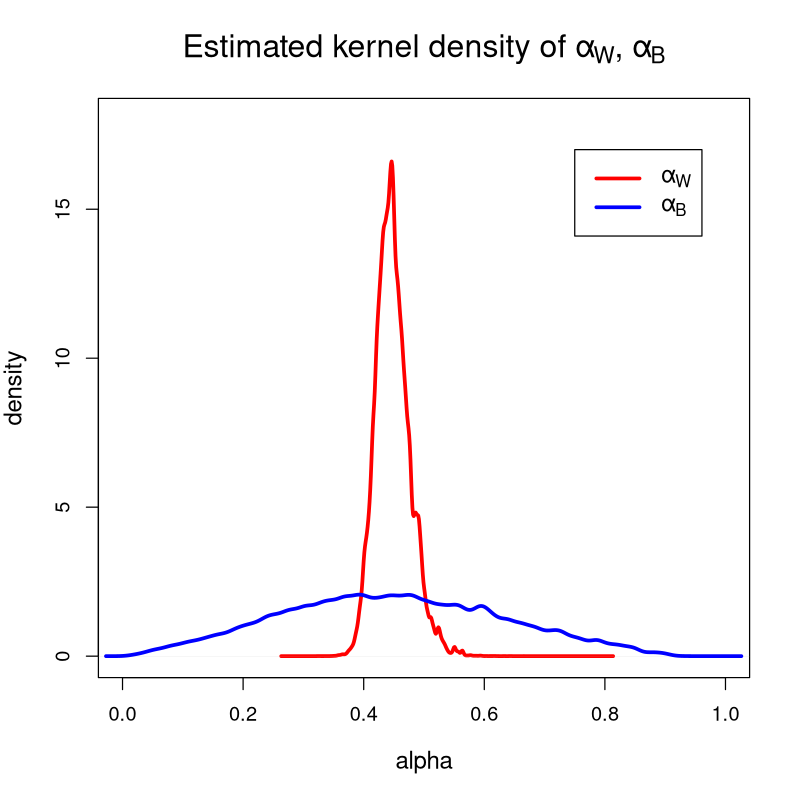
\includegraphics[width=\textwidth]{./distributions.png}

Interestingly, the density at $\alpha_W=\alpha_B=1$ is almost $0$.
This might suggest that no players are playing perfectly optimally, but more likely than not,
this indicates one of the flaws of the Elo rating system.

It is clearly useful (and very effective) for ranking players, but does poorly when applied
to draw prediction. This is not relevant for its main purpose, but poses a challenge here.
Because the Elo expected value $$E_W=\pw + \frac{1}{2}\pd$$
neither defines $\pw$ nor $\pd$, instead assigning a ``payoff'' of $\frac{1}{2}$ to drawing,
it becomes difficult to predict draw behavior using it.
This is especially visible at high levels of play where draws are quite common;
35\% of games in the cleaned dataset were draws.
This flaw was also present in the
modified Elo expected value, which was more to
derive relative playing strength in the form of adjusted ratings, rather than directly compute draw probabilities.

So rather than looking at the individual distributions of $\alpha_W,\alpha_B$, it is more informative to examine
the distribution of their difference.

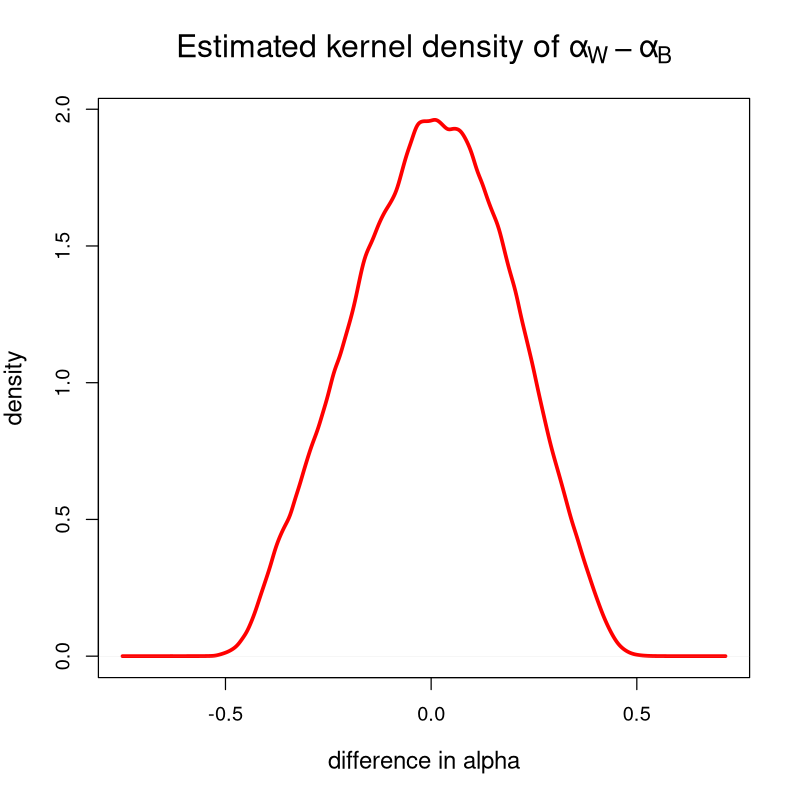
\includegraphics[width=\textwidth]{./diff.png}

This is almost zero-mean, with the average difference being $0.0015$ and the median difference being $0.0055$.
It should be expected that white plays less passively, since white wins 37\% of the time as compared
to black's 28\%
(in this dataset).
Interestingly the tails of the $\alpha_B$ distribution are quite long in comparison to the short tails of the $\alpha_W$ distribution.
This could again be due to black's native disadvantage encouraging more deviation and more strategies chosen
to either really attempt to win (higher $\alpha_B$) or attempt to draw at at all costs (lower $\alpha_W$).

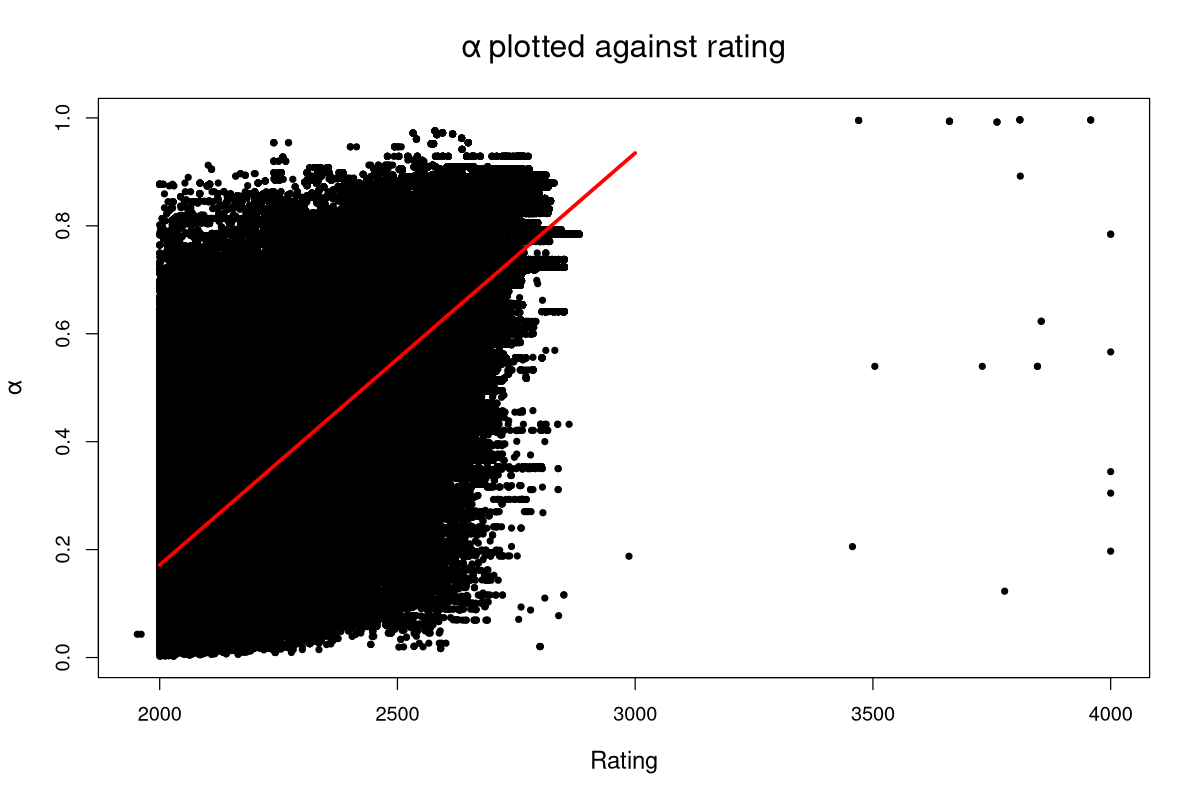
\includegraphics[width=\textwidth]{./linear.png}

There is also a correlation between rating and $\alpha$, with an $R$-value of 0.5047, indicating that at higher ratings
there is less suboptimal play.
This is not totally unsurprising, since at the highest echelons of play this suboptimal playing behavior is much more easily
observed, socially discouraged, and more heavily punished by other players (due to the higher levels of play).
At slightly lower levels of play, from national masters to lower-rated international masters, though, we observe lower
values of $\alpha$.

\section{Conclusion}
These results relate back to the article/real-world situation in a couple of ways.
First, it shows that variance-lowering behavior at the cost of expected value does occur in chess.
That is, playing suboptimally for draws at higher levels of play occurs often.
It is difficult to identify, however, if this is as a result of random noise or variance in playing strength
on behalf of players, or if each choice of $\alpha_W, \alpha_B$ for each game is intentional.
It is also clear that this behavior, on average, decreases as the level of play increases, as predicted.

That being said, the majority of situations involve players playing similarly, that is choosing
$\alpha_W\approx \alpha_B$, so although some suboptimal hyperpassive play occurs, it does not occur
sufficiently to pose a threat to the integrity of the game.

The article mentions measures designed to increase errors and decrease the likelihood of draws.
These would likely be successful at the highest echelons of play, where games are sufficiently
scrutinized and play is so precise that suboptimal play essentially does not exist.
However, at slightly lower levels of play (still professional, but just among weaker players), the problem is not absolute precision.
Rather, (assuming the results support this), the problem is this variance-reducing behavior.
So from a design perspective, the solution would be to penalize this behavior.
Making draws worth $\frac{1}{3}$ of a point could discourage taking draws in tournaments, for instance.
Removing agreed draws (where players simply agree to a draw rather than playing it out) as a whole could also make this behavior more difficult.

% TODO BIB
Caissabase, Elo, Smerdon, The Fuzz, original article
\end{document}
